%%%%%%%%%%%%%%%%%%%%%%%%%%%%%%%%%%%%%%%%%%%%%%%%%%%%%%%%%%%%%%%%%%%%%%%%%%%%%%%
\section{Biased Eigenvalues in Heterogeneous Geometries}
\label{sec:bias}
%%%%%%%%%%%%%%%%%%%%%%%%%%%%%%%%%%%%%%%%%%%%%%%%%%%%%%%%%%%%%%%%%%%%%%%%%%%%%%%


\begin{equation}
\label{eqn:delta-rho}
\Delta\rho = \left(k_{eff}^{OpenMOC} - k_{eff}^{OpenMC}\right) \times 10^{5}
\end{equation}

-data is for 2D fuel pin with MGXS tallied by FSR

\begin{table}[h!]
  \centering
  \caption{Reference OpenMC eigenvalues for a 2D fuel pin.}
  \label{table:keff-reference} 
  \begin{tabular}{c c}
  \toprule
  {\bf Anisotropic} &
  {\bf Isotropic in Lab} \\
  \midrule
  1.17486 $\pm$ 0.00003 & 1.17421 $\pm$ 0.00002 \\
  \bottomrule
\end{tabular}
\end{table}

\begin{table}[h!]
  \centering
  \caption{The eigenvalue bias with transport-corrected MGXS.}
  \label{table:keff-bias-aniso} 
  \begin{tabular}{c S[table-format=6.1] S[table-format=6.1] S[table-format=6.1]}
  \toprule
  & \multicolumn{3}{c}{{\bf FSR Discretization}} \\
  \midrule
  \multicolumn{1}{c}{{\bf \# Groups}} &
  {\bf 1$\times$} & {\bf 4$\times$} & {\bf 16$\times$} \\
  \midrule
1 & 53 & 75 & 72 \\
2 & 37 & 1 & 4 \\
4 & -58 & -92 & -109 \\
8 & -74 & -145 & -170 \\
16 & -67 & -154 & -183 \\
25 & -124 & -221 & -245 \\
40 & -130 & -238 & -265 \\
70 & -131 & -281 & -274 \\
  \bottomrule
\end{tabular}
\end{table}


\begin{table}[h!]
  \centering
  \caption{The eigenvalue bias with isotropic-in-lab scattering.}
  \label{table:keff-bias-iso-in-lab} 
  \begin{tabular}{c S[table-format=6.1] S[table-format=6.1] S[table-format=6.1]}
  \toprule
  & \multicolumn{3}{c}{{\bf FSR Discretization}} \\
  \midrule
  \multicolumn{1}{c}{{\bf \# Groups}} &
  {\bf 1$\times$} & {\bf 4$\times$} & {\bf 16$\times$} \\
  \midrule
1 & 80 & 55 & 66 \\
2 & 141 & 29 & 34 \\
4 & 27 & -43 & -57 \\
8 & 26 & -85 & -102 \\
16 & 35 & -91 & -111 \\
25 & -31 & -158 & -182 \\
40 & -38 & -174 & -202 \\
70 & -39 & -182 & -211 \\
  \bottomrule
\end{tabular}
\end{table}


\begin{itemize}
\item Slab problem -- horrible flux shape and eigenvalue!!
\item Pin-Cell
\item Plot showing bias is driven by resonance groups
\item Simple 1-group fixed source demonstration
\end{itemize}


%%%%%%%%%%%%%%%%%%%%%%%%%%%%%%%%%%%%%%%%%%%%%%%%%%%%%%%%%%%%%%%%%%%%%%%%%%%%%%%
\section{Diagnosis of Bias}
%%%%%%%%%%%%%%%%%%%%%%%%%%%%%%%%%%%%%%%%%%%%%%%%%%%%%%%%%%%%%%%%%%%%%%%%%%%%%%%

\begin{figure}[h!]
\centering
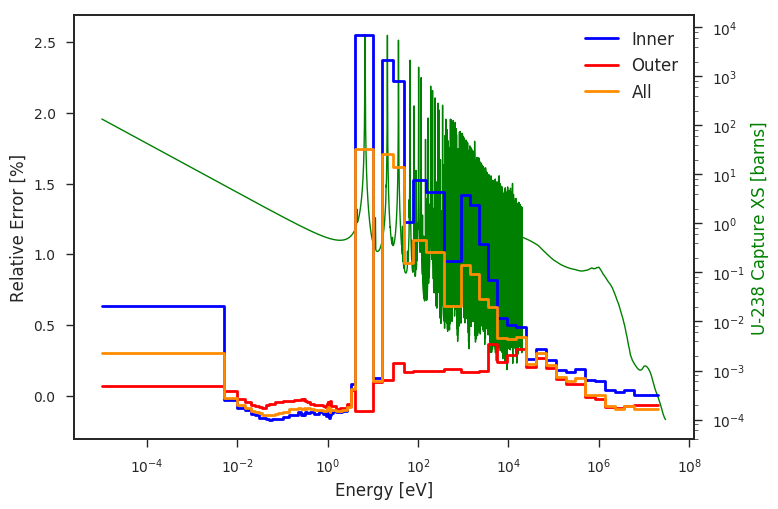
\includegraphics[width=\linewidth]{figures/rel-err-inner-outer}
\caption{The energy-dependent relative error of the OpenMOC scalar flux with respect to the reference OpenMC flux for the innermost, outermost and all FSRs.}
\label{fig:rel-err-energy}
\end{figure}

\begin{figure}[H]
\centering
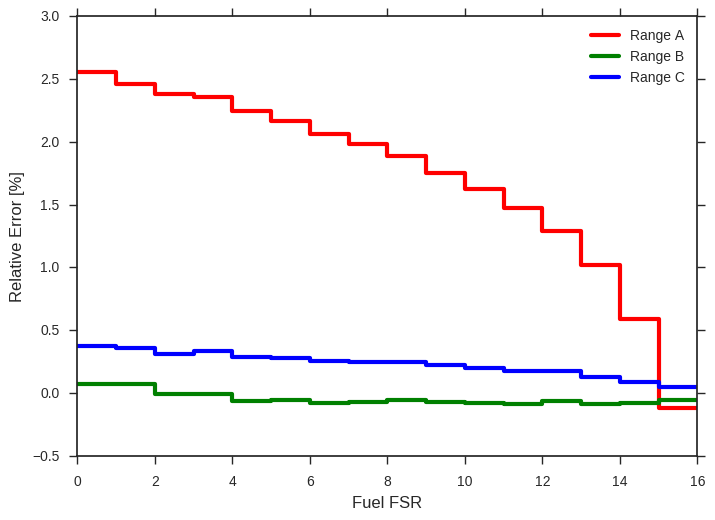
\includegraphics[width=0.8\linewidth]{figures/rel-err-fuel-fsrs}
\caption{The spatially-varying relative error of the OpenMOC scalar flux with respect to the reference OpenMC flux in energy Ranges A, B, and C.}
\label{fig:rel-err-space}
\end{figure}

\begin{itemize}
\item Assert that angular effects drive the bias
\item Evidenced by small effect on bias from:
\begin{itemize}
\item Isotropic vs. Anisotropic LAB scattering
\item Spatial mesh refinement
\end{itemize}
\item Demonstrate angular dependent cross sections remove bias
\begin{itemize}
\item Pin-Cell
\item Slab
\end{itemize}
\item Show angular dependent cross section plots
\end{itemize}
